\documentclass{beamer}
\usepackage{amsmath}
\usepackage{graphicx}
\usepackage{subfigure}
\usepackage{xcolor}
%\usepackage{tcolorbox}

%\usepackage{caption}
%\usepackage{subcaption}

% Copyright 2004 by Till Tantau <tantau@users.sourceforge.net>.
%
% In principle, this file can be redistributed and/or modified under
% the terms of the GNU Public License, version 2.
%
% However, this file is supposed to be a template to be modified
% for your own needs. For this reason, if you use this file as a
% template and not specifically distribute it as part of a another
% package/program, I grant the extra permission to freely copy and
% modify this file as you see fit and even to delete this copyright
% notice. 


\mode<presentation>
{
  \usetheme{default}
  % or ...

  \setbeamercovered{transparent}
  % or whatever (possibly just delete it)
}


\usepackage[english]{babel}
% or whatever

\usepackage[utf8]{inputenc}
% or whatever

\usepackage{xcolor}
\usepackage[percent]{overpic}

\usefonttheme{serif}
\usecolortheme{seahorse}

\usepackage[T1]{fontenc}

\title[CIPANP Vail, CO]
{ADMX Status Update}

\author[Malagon]
{Ana Malag\'on}

\institute[University of Washington]
{University of Washington, ADMX Collaboration}

\date[May 23, 2015]
{May 23, 2015/CIPANP Vail, CO}

\begin{document}

\begin{frame}
\titlepage
\end{frame}

\begin{frame}{Outline}
\begin{enumerate}
\item The Strong CP Problem\medskip
\item Axion as Dark Matter\medskip
\item The Experiment\medskip
\item Upgrades for Gen2\medskip
\item Research In Progress\medskip
\end{enumerate}

\end{frame}

\begin{frame}{Strong CP Problem}
\begin{align*}
\mathcal{L}_{QCD} = \frac{\theta}{32 \pi}G\tilde G
\end{align*}

\begin{enumerate}
\item $\theta$ exactly cancels CP violating phase from CKM matrix so that CP-violating observable $\bar{\theta} < 10^{-10}$ (limit from null observations of neutron EDM).\medskip
\item Why is that?

\end{enumerate}

\end{frame}

%\usebackgroundtemplate{%
%  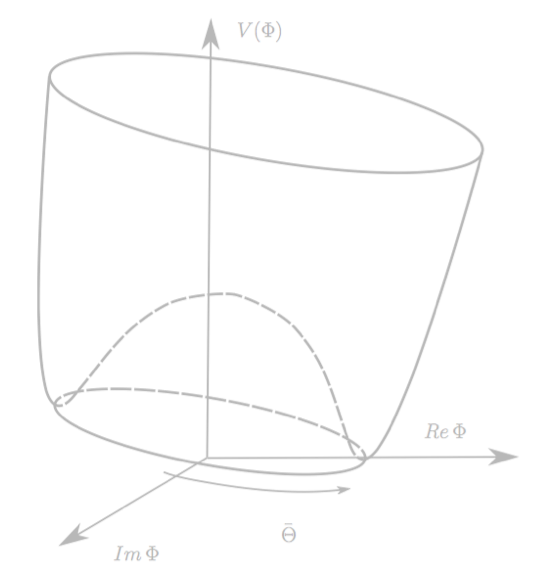
\includegraphics[width=\paperwidth,height=\paperheight]{wine_bottle_transparent}} 

\begin{frame}{Peccei-Quinn Mechanism}
\begin{enumerate}
\item Introduce a new global chiral symmetry: $U(1)_{PQ}$
\item The Goldstone boson of the broken symmetry is a massless axion: $a(x)$.
\item Anomalies of the symmetry with QCD introduce a potential for $a(x)$ {\tiny (and therefore a small mass, $m_a \propto f_a^{-1}$)}: 
\begin{align*}
\frac{a(x)}{f_a}G\tilde G
\end{align*}
\item The minimum value of the total potential from $\bar{\theta}$ and $a(x)$ gives $\langle a(x)/f_a - \bar{\theta} \rangle = 0$.
\end{enumerate}

This is not the only solution to the strong CP problem, but provides a testable low energy observable: the axion.
\end{frame}

\begin{frame}{Axion as Dark Matter}
\begin{enumerate}
\item The effects of the potential
\begin{align*}
\frac{a(x)}{f_a}G\tilde G
\end{align*}
only become important after energy scales are less than $\Lambda_{QCD}$.
\item Therefore at higher energies the initial value of $a(x)$ can be 
``misaligned'' from $\langle a(x) \rangle = \bar{\theta}$.
\item This initial misalignment of the field provides a primordial energy density of axions.
\item If this primordial population is feebly interacting, stable, and cold, it could be dark matter.
\end{enumerate}

\end{frame}

%\begin{frame}{Axion: what is it?}
%\begin{itemize}
%\item dark matter candidate
%\item could explain why CP violation is so small in QCD
%\item low energy observable of high energy scales
%\end{itemize}
%\end{frame}

\begin{frame}{Dark Matter Axion: where is it?}
\textit{Between 1 $\mu$eV\footnote{this is a very squishy bound} and 1 meV, roughly.}\\
{\tiny {\color{blue} corresponds to $10^9$ GeV $\leq f_a \leq 10^{12}$ GeV.}}\medskip
%QCD axion has magical properties:
%\begin{enumerate}
%\item coupling $g$ proportional to mass $m_a$
%\item both inversely proportional to energy scale of symmetry breaking $f_a$
%\item there is a generic coupling to two photons (like pion); this comes out in Lagrangian as $L_I = gE\cdot B$
%\end{enumerate}

Axion coupling to two photons $g_{a\gamma\gamma}$ predicted to be:
\begin{description}
\item[ ] KSVZ:  $|g_{a\gamma\gamma}| = 0.002 / f_a$ $\text{GeV}^{-1}$
\item[ ] DFSZ: $|g_{a\gamma\gamma}| = 0.008 / f_a$ $\text{GeV}^{-1}$
\end{description}
\begin{columns}
\column{0.5\textwidth}
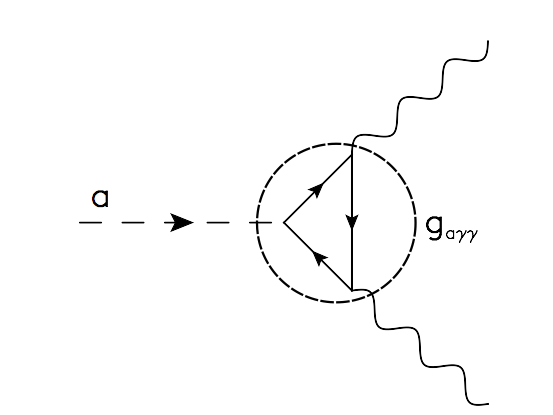
\includegraphics[width=\textwidth]{axion_photon_feynman_diagram}
\column{0.5\textwidth}

{\tiny For $m_a =10^{-5}$ eV dark matter axion:}

{\tiny Number Density: {\color{red} $10^{16}/\text{Liter}$}}

{\tiny DeBroglie Coherence Length: {\color{red} 100 m}}

{\tiny Energy Resolution $\Delta E_a:  10^{-6}m_a$ }

{\tiny Frequency of Corresponding Photon: {\color{blue} 2.4 GHz }}
\end{columns}
\end{frame}

\begin{frame}{Experimental Handles}

 \begin{description}
\item[ ] \textsc{Microwave Cavity Searches}: {\tiny $g_{a\gamma\gamma}^2$}
\begin{description}
\item[ ]  ADMX
\item[ ]  ADMX-HF
\item[ ]  KAIST
\end{description}

\item[ ] \textsc{Photon Regeneration}: {\tiny $g_{a\gamma\gamma}^4$}
\begin{description}
\item[ ]  ALPs-II
\end{description}
\item[ ] \textsc{Solar Axion Searches}: {\tiny $g_{a\gamma\gamma}^4$}
\begin{description}
\item[ ]  CAST 
\end{description}
\item[ ] \textsc{Macroscopic Spin Forces}: {\tiny $g_S g_P$}
\begin{description}
\item[ ]  Eot-Wash {\tiny (torsion pendulum)}
\item[] ARIADNE {\tiny (polarized He$^3$)}
\end{description}
\item[ ] \textsc{Oscillating EDMs}: {\tiny $g_{aNN}^2$}
\begin{description}
\item[ ]  CASPER
\end{description}
\end{description}
\end{frame}

\begin{frame}{Signal}
\begin{columns}
\column{.32\textwidth}
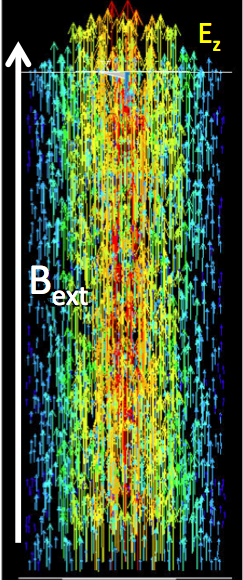
\includegraphics[width=\textwidth]{colorful_cavity}
\column{0.68\textwidth}
\begin{center}
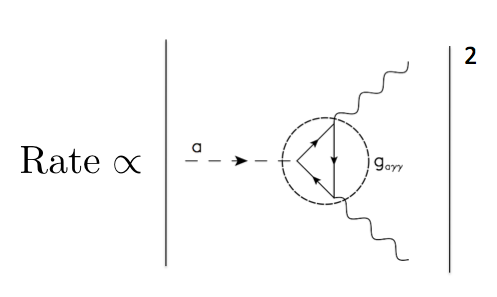
\includegraphics[width=.55\textwidth]{rate} 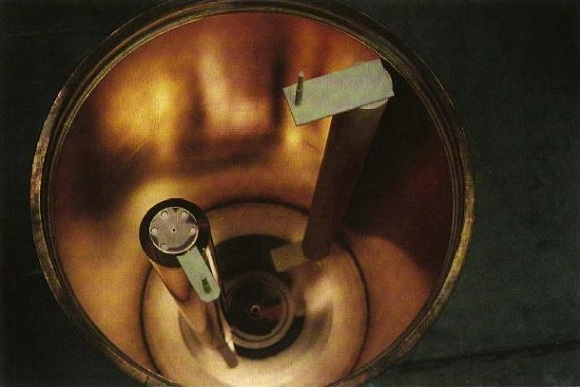
\includegraphics[width=0.5\textwidth]{cavity_open}

\end{center}
\begin{align*}
\mathcal{L}_I = - \frac{1}{4}g_{a\gamma \gamma}aF\tilde F = g_{a\gamma \gamma}a\vec{E}\cdot\vec{B}
\end{align*}
\begin{align*}
\text{Signal Power} = g_{a\gamma \gamma}^2 a^2 [B_{\text{ext}}^2 V] C Q
\end{align*}
%\begin{columns}
%\column{.4\textwidth}
$g_{a\gamma\gamma}$ - {\tiny coupling constant} \quad $B_{ext}$ - {\tiny external magnetic field}\\
$m_a a^2 = \rho_a$ {\tiny local dark matter energy density}
%\column{.4\textwidth}
$V$ - {\tiny volume}\\ C = {\tiny $\mathcal{O}(1)$} {\tiny form factor} \qquad
$Q$ - {\tiny quality factor}
%\end{columns}
\end{columns}
\end{frame}

\begin{frame}{Noise}
{\tiny Background = Johnson Noise of Cavity + Noise from Electronics}
\begin{center}
$\text{System Temperature} = T_{cavity} + T_{amp}$

$\text{Statistical Fluctuations: } \Delta T = \frac{T_{system}}{\sqrt{\tau BW_{\text{a}}}}$
\end{center}

 {\tiny $\rightarrow$ To reach KSVZ sensitivity @ averaging times of $\tau = 100$ s, stepped by $\mathcal{O}(1\%)$ of $\text{cavityBW}$.}
 
 \begin{columns}
\column{0.36\textwidth}
{\tiny {\color{blue} 2014 run temperatures}}
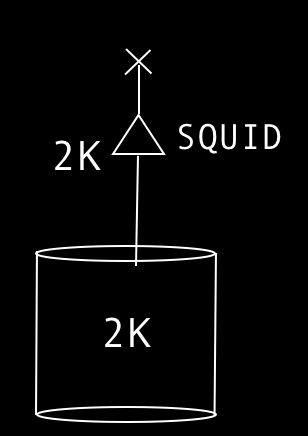
\includegraphics[width=\textwidth]{dark_2K}
\column{0.32\textwidth}{\tiny microstrip squid amplifier}
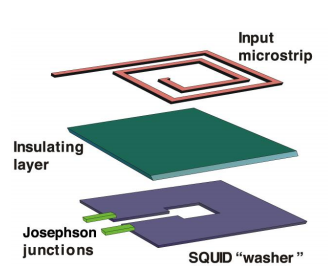
\includegraphics[width=\textwidth]{msa_exploded_view}

\column{0.3\textwidth}
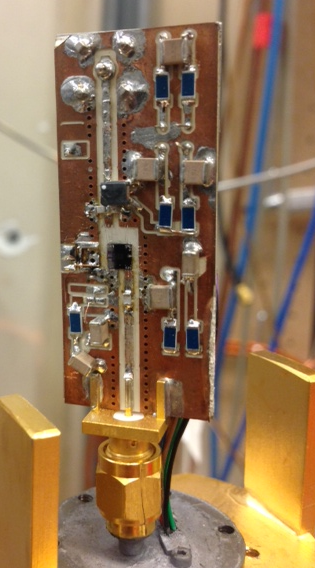
\includegraphics[width=\textwidth]{squid_exposed}
\end{columns}
\end{frame}

\begin{frame}{Magnet}
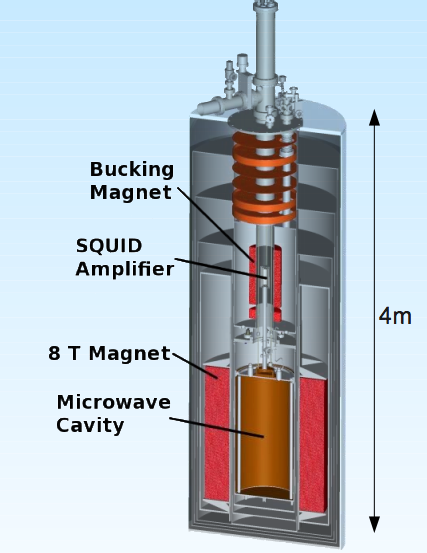
\includegraphics[width=0.5\textwidth]{admx_schematic} \quad 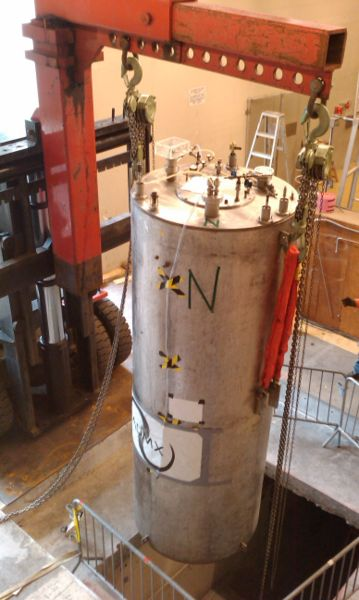
\includegraphics[width=0.4\textwidth]{magnet_lowered}

\end{frame}

\begin{frame}{Insert}
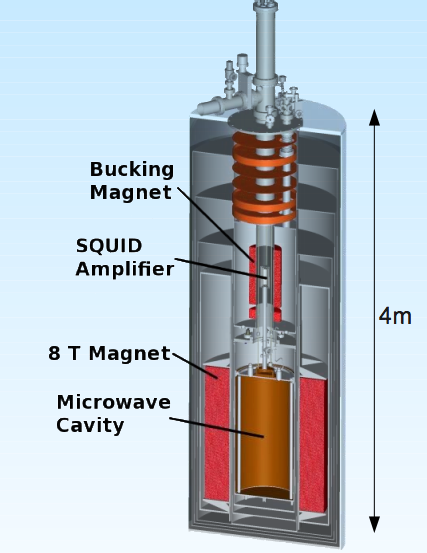
\includegraphics[width=0.5\textwidth]{admx_schematic} \quad 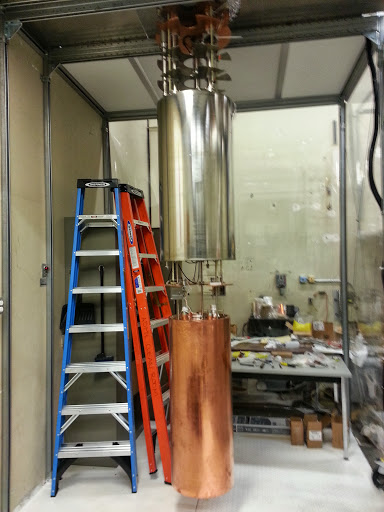
\includegraphics[width=0.45\textwidth]{cavity_hanging}
\end{frame}

\begin{frame}{Insert}
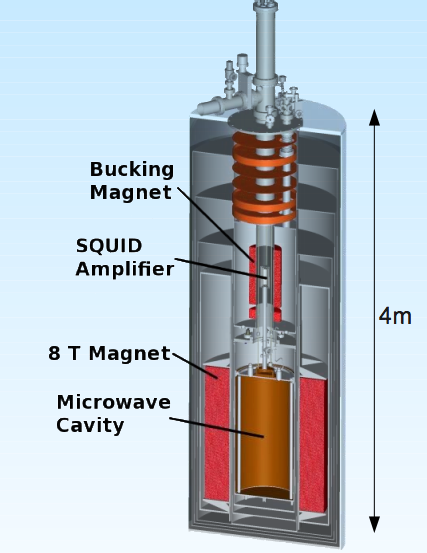
\includegraphics[width=0.5\textwidth]{admx_schematic} \quad 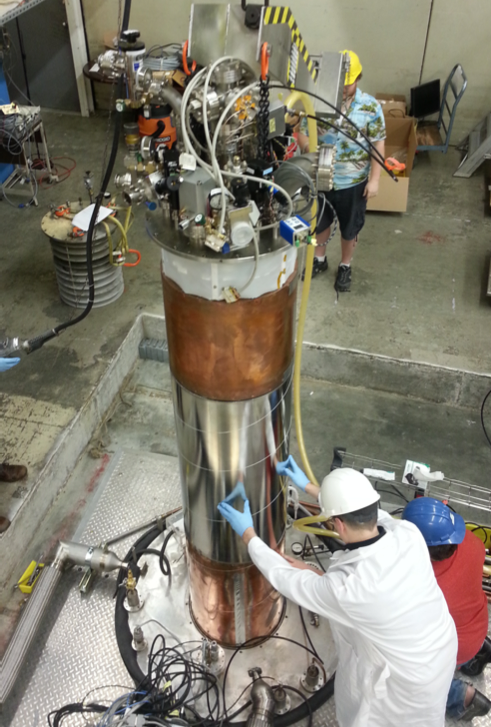
\includegraphics[width=0.45\textwidth]{lowering_insert}

\end{frame}

\begin{frame}{Experimental Site}
\includegraphics[width=\textwidth]{boutan_photo4}
\end{frame}

%\begin{frame}{Axion Dark Matter Experiment}
%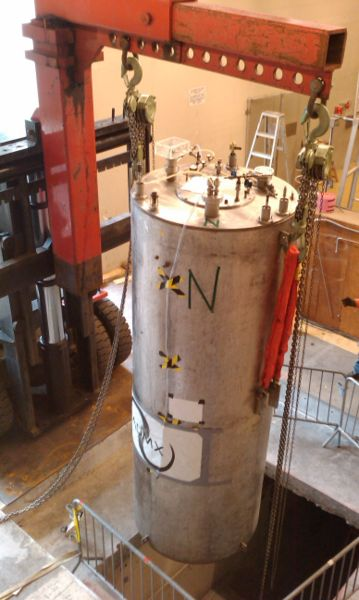
\includegraphics[width=0.5\textwidth]{magnet_lowered}
%
%%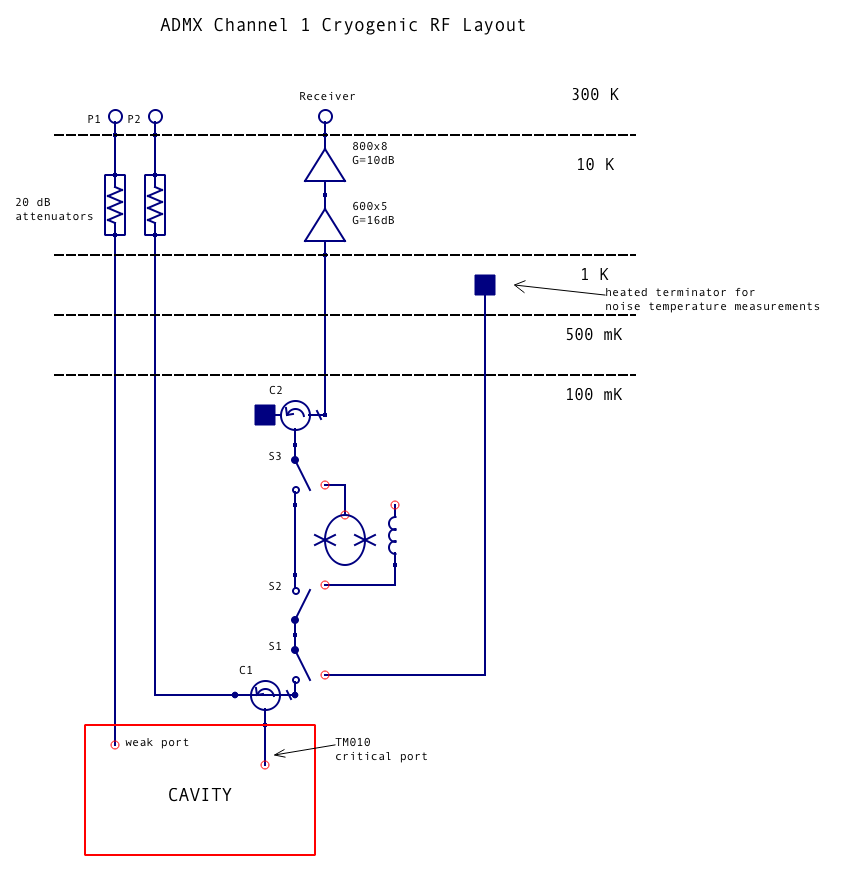
\includegraphics[width=.8\textwidth]{export_cryo_layout_msa_text}
%\end{frame}



%\begin{frame}{Background}
%Johnson noise from cavity plus electronic noise (dominated by first amplifier)
%Background is fluctuations in noise power. Are proportional to system noise temperature and inversely proportional to the square root of the averaging time.
%
%Dil Fridge
%Quantum-Limited Amplifiers
%%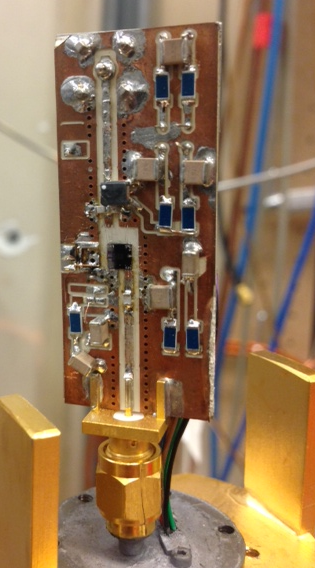
\includegraphics[width=0.3\textwidth]{squid_exposed}
%\end{frame}

\begin{frame}{Results from 2014}
\begin{columns}
\column{0.5\textwidth}
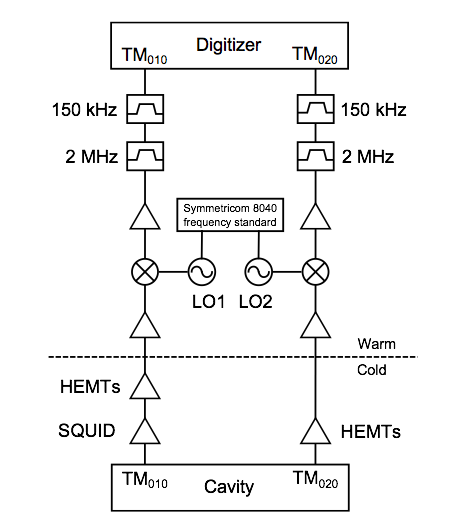
\includegraphics[width=\textwidth]{two_channel_diagram}
\column{0.5\textwidth}
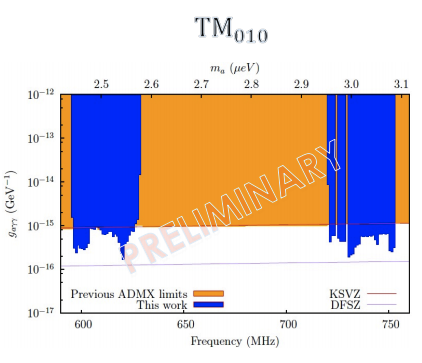
\includegraphics[width=.9\textwidth]{2014_results_1}

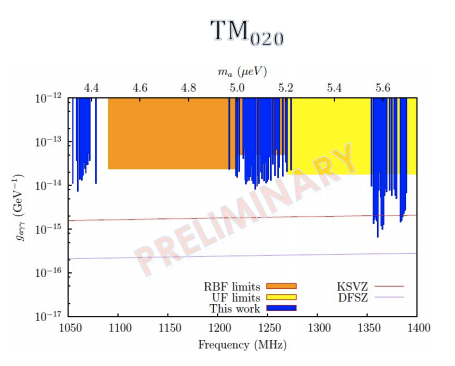
\includegraphics[width=.95\textwidth]{2014_results_2}
\end{columns}
\end{frame}

\begin{frame}{Upgrades for Gen2}

{\color{red} \textbf{\large{Dilution Refrigerator}}}: $T_{system} \approx 200$ mK.
\begin{columns}
\column{0.5\textwidth}
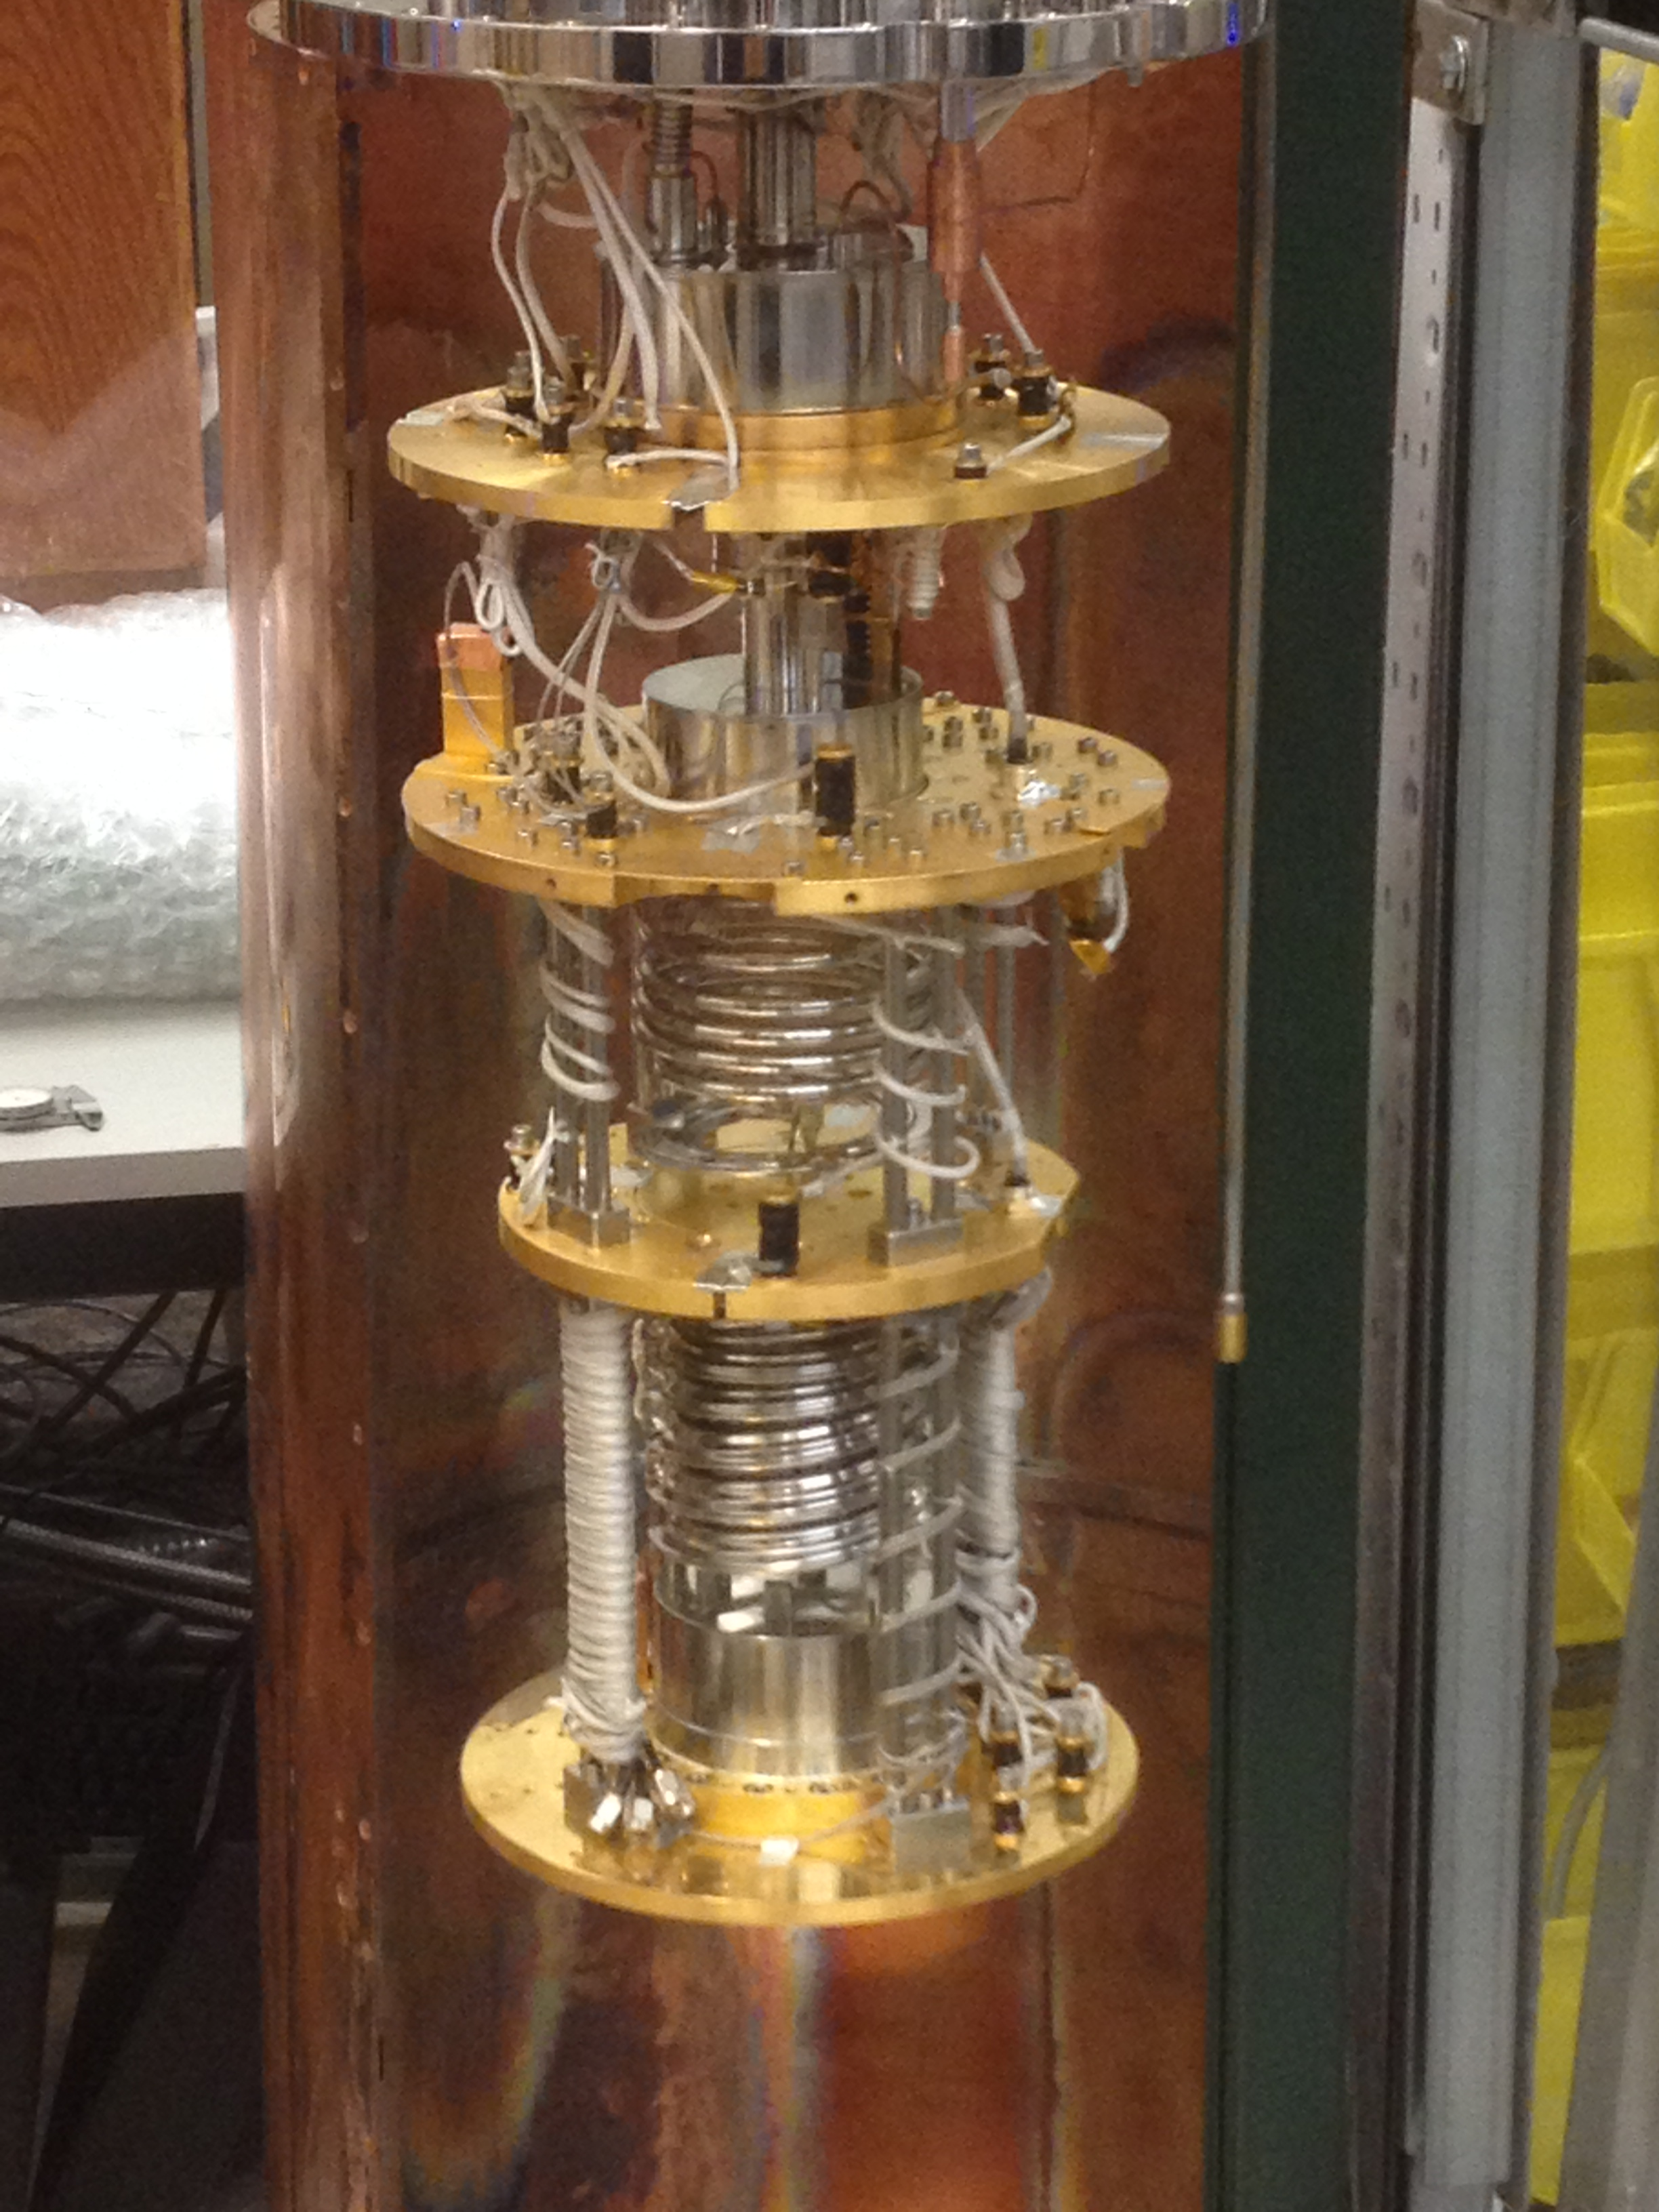
\includegraphics[width=\textwidth]{dil_fridge_glamour_shot}
\column{0.5\textwidth}
- Arrived March 30th.

- Plan to turn on to begin tests of $<$Kelvin temps in two weeks.\medskip

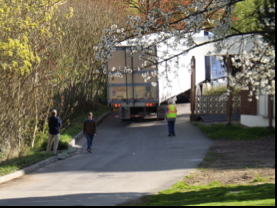
\includegraphics[width=\textwidth]{semi}

\end{columns}

\end{frame}

\begin{frame}{Upgrades for Gen2}

\textbf{JPA} on second channel.
\begin{columns}
\column{0.5\textwidth}
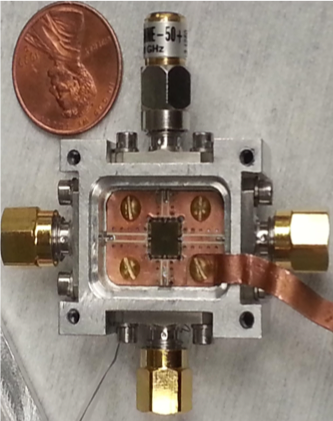
\includegraphics[width=\textwidth]{jpa_exposed}
\column{0.5\textwidth}\textbf{Sidecar} @ 3.9+ GHz, {\tiny will be able to reach $g \simeq 10^{-14}$ GeV$^{-1}$}
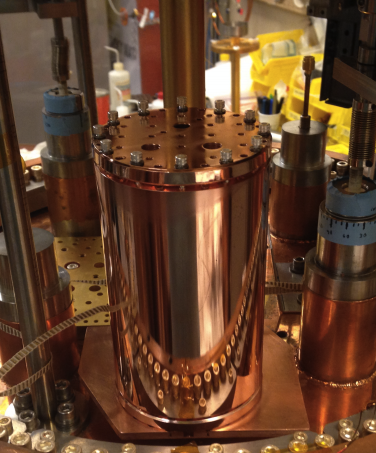
\includegraphics[width=\textwidth]{sidecar_single}
\end{columns}

\end{frame}

%\begin{frame}
%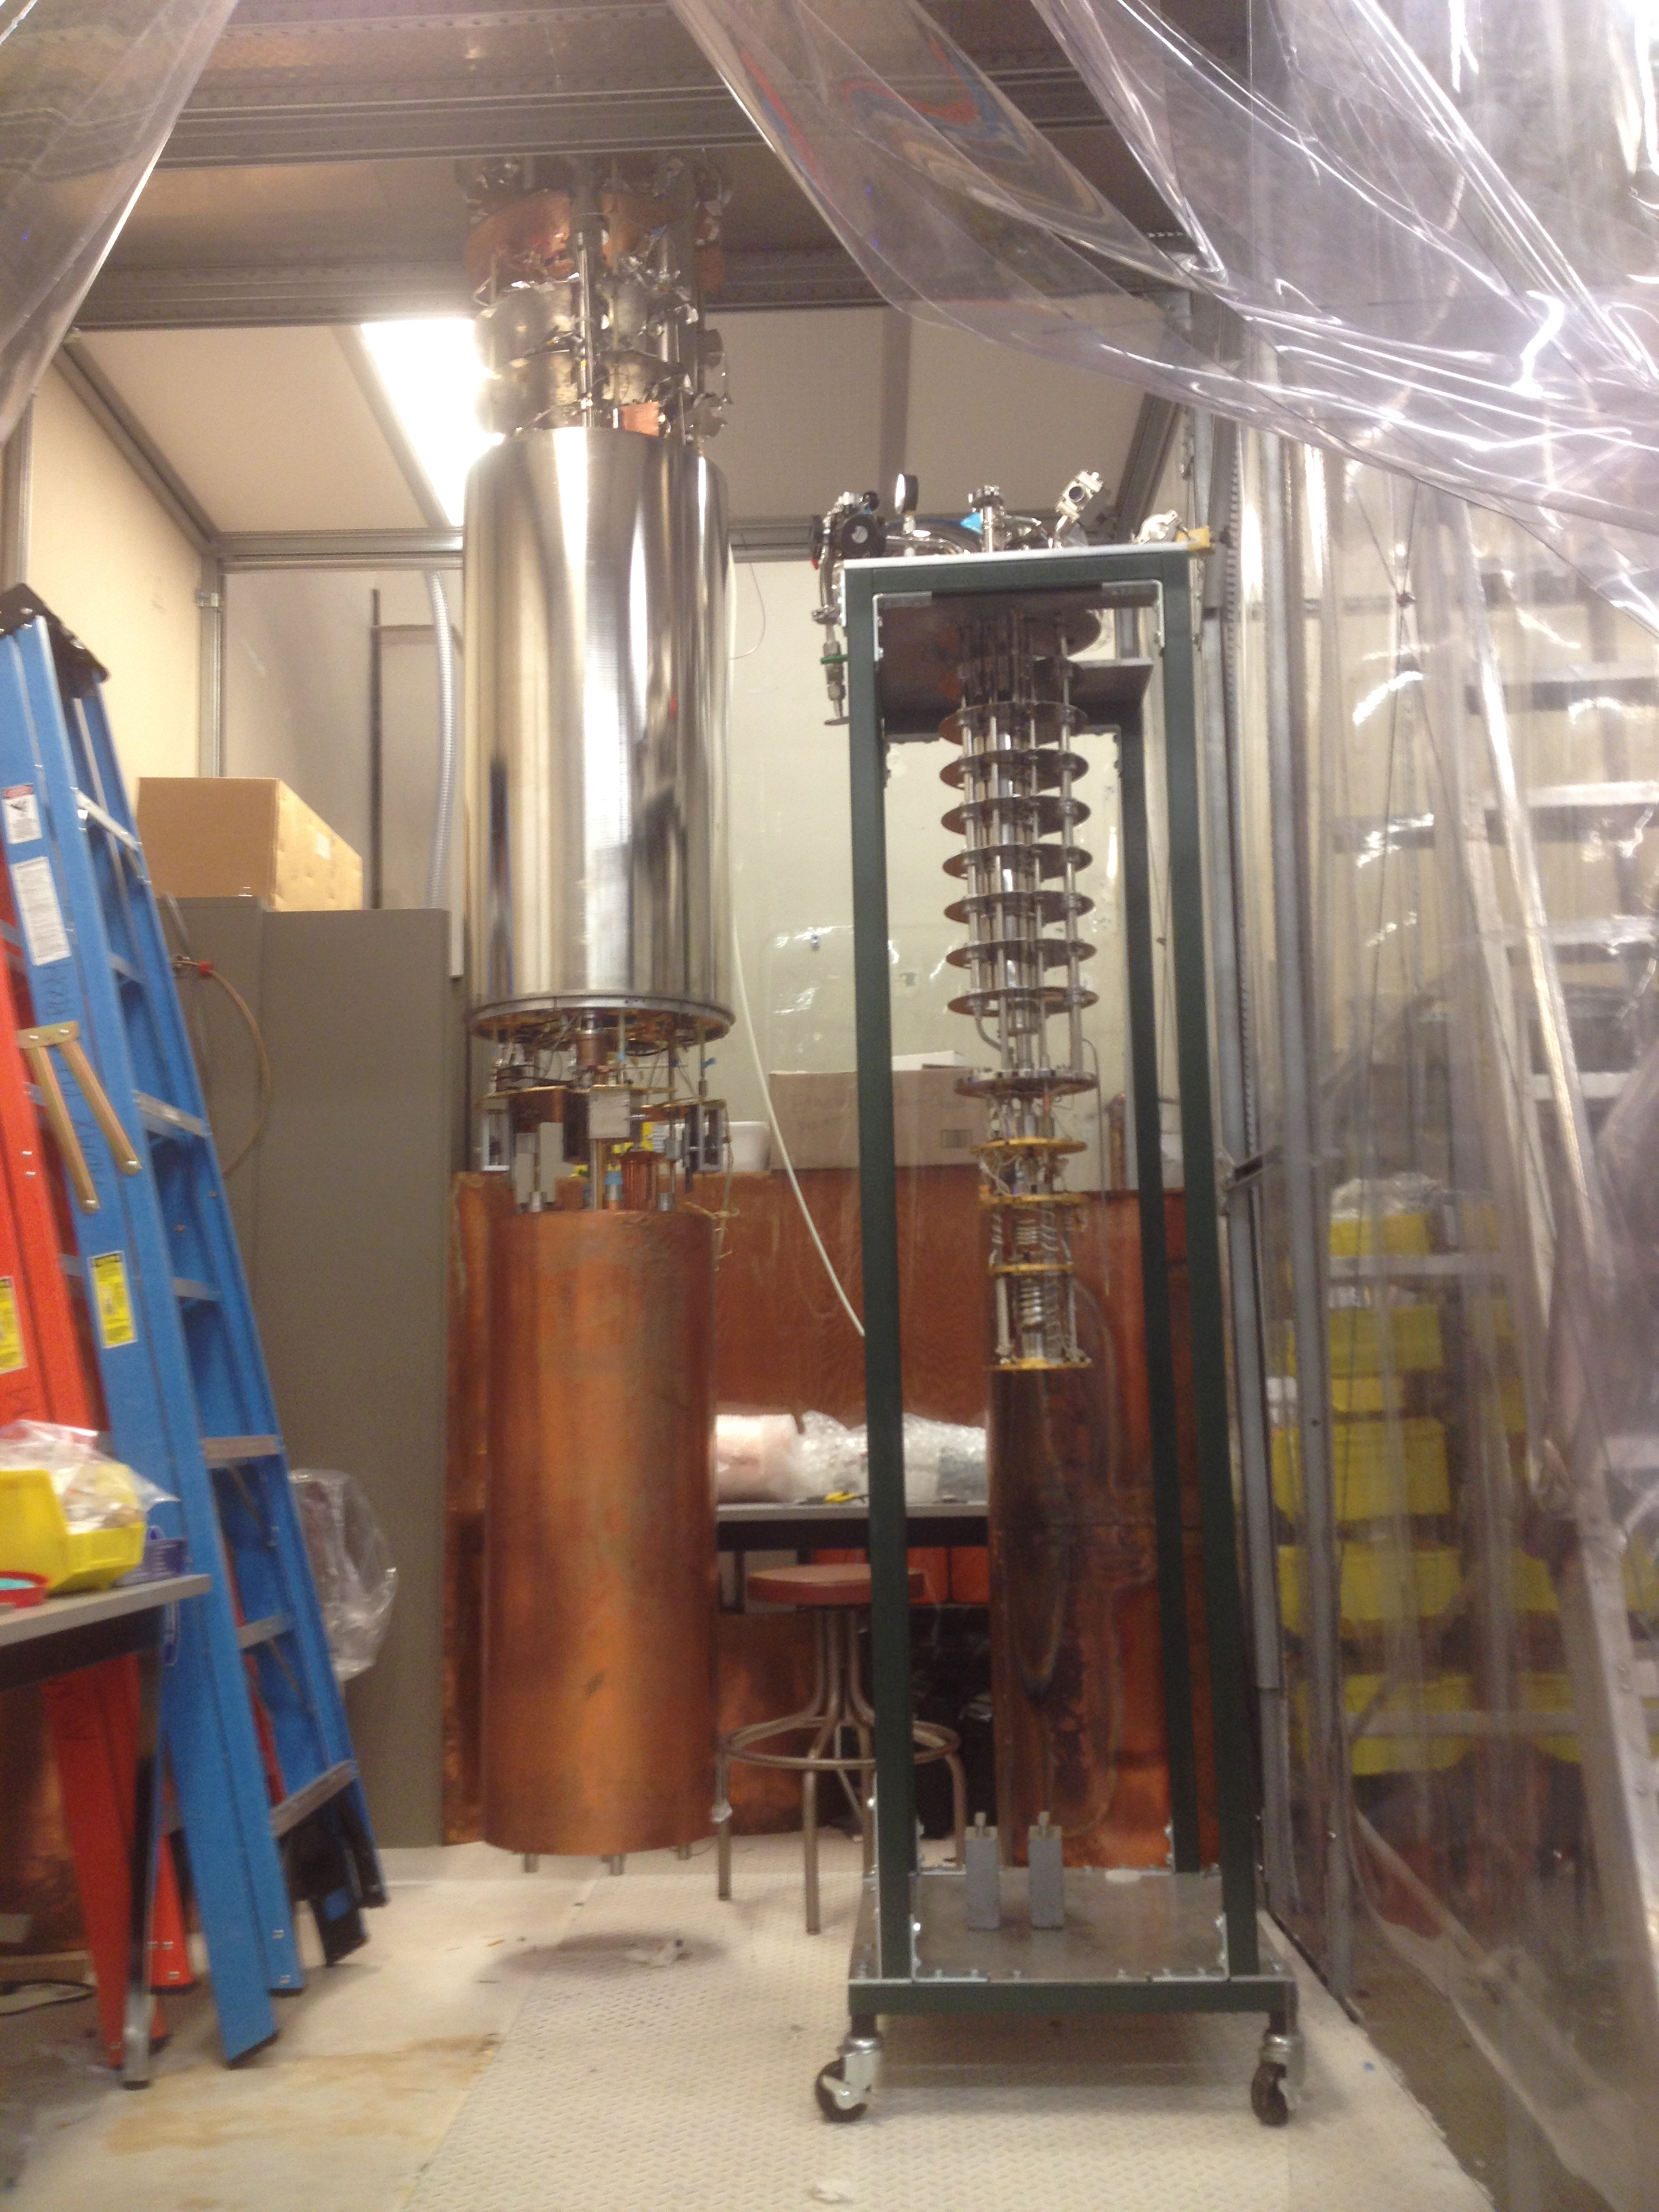
\includegraphics[width=0.5\textwidth]{cleanroom_cavity_dilfridge}
%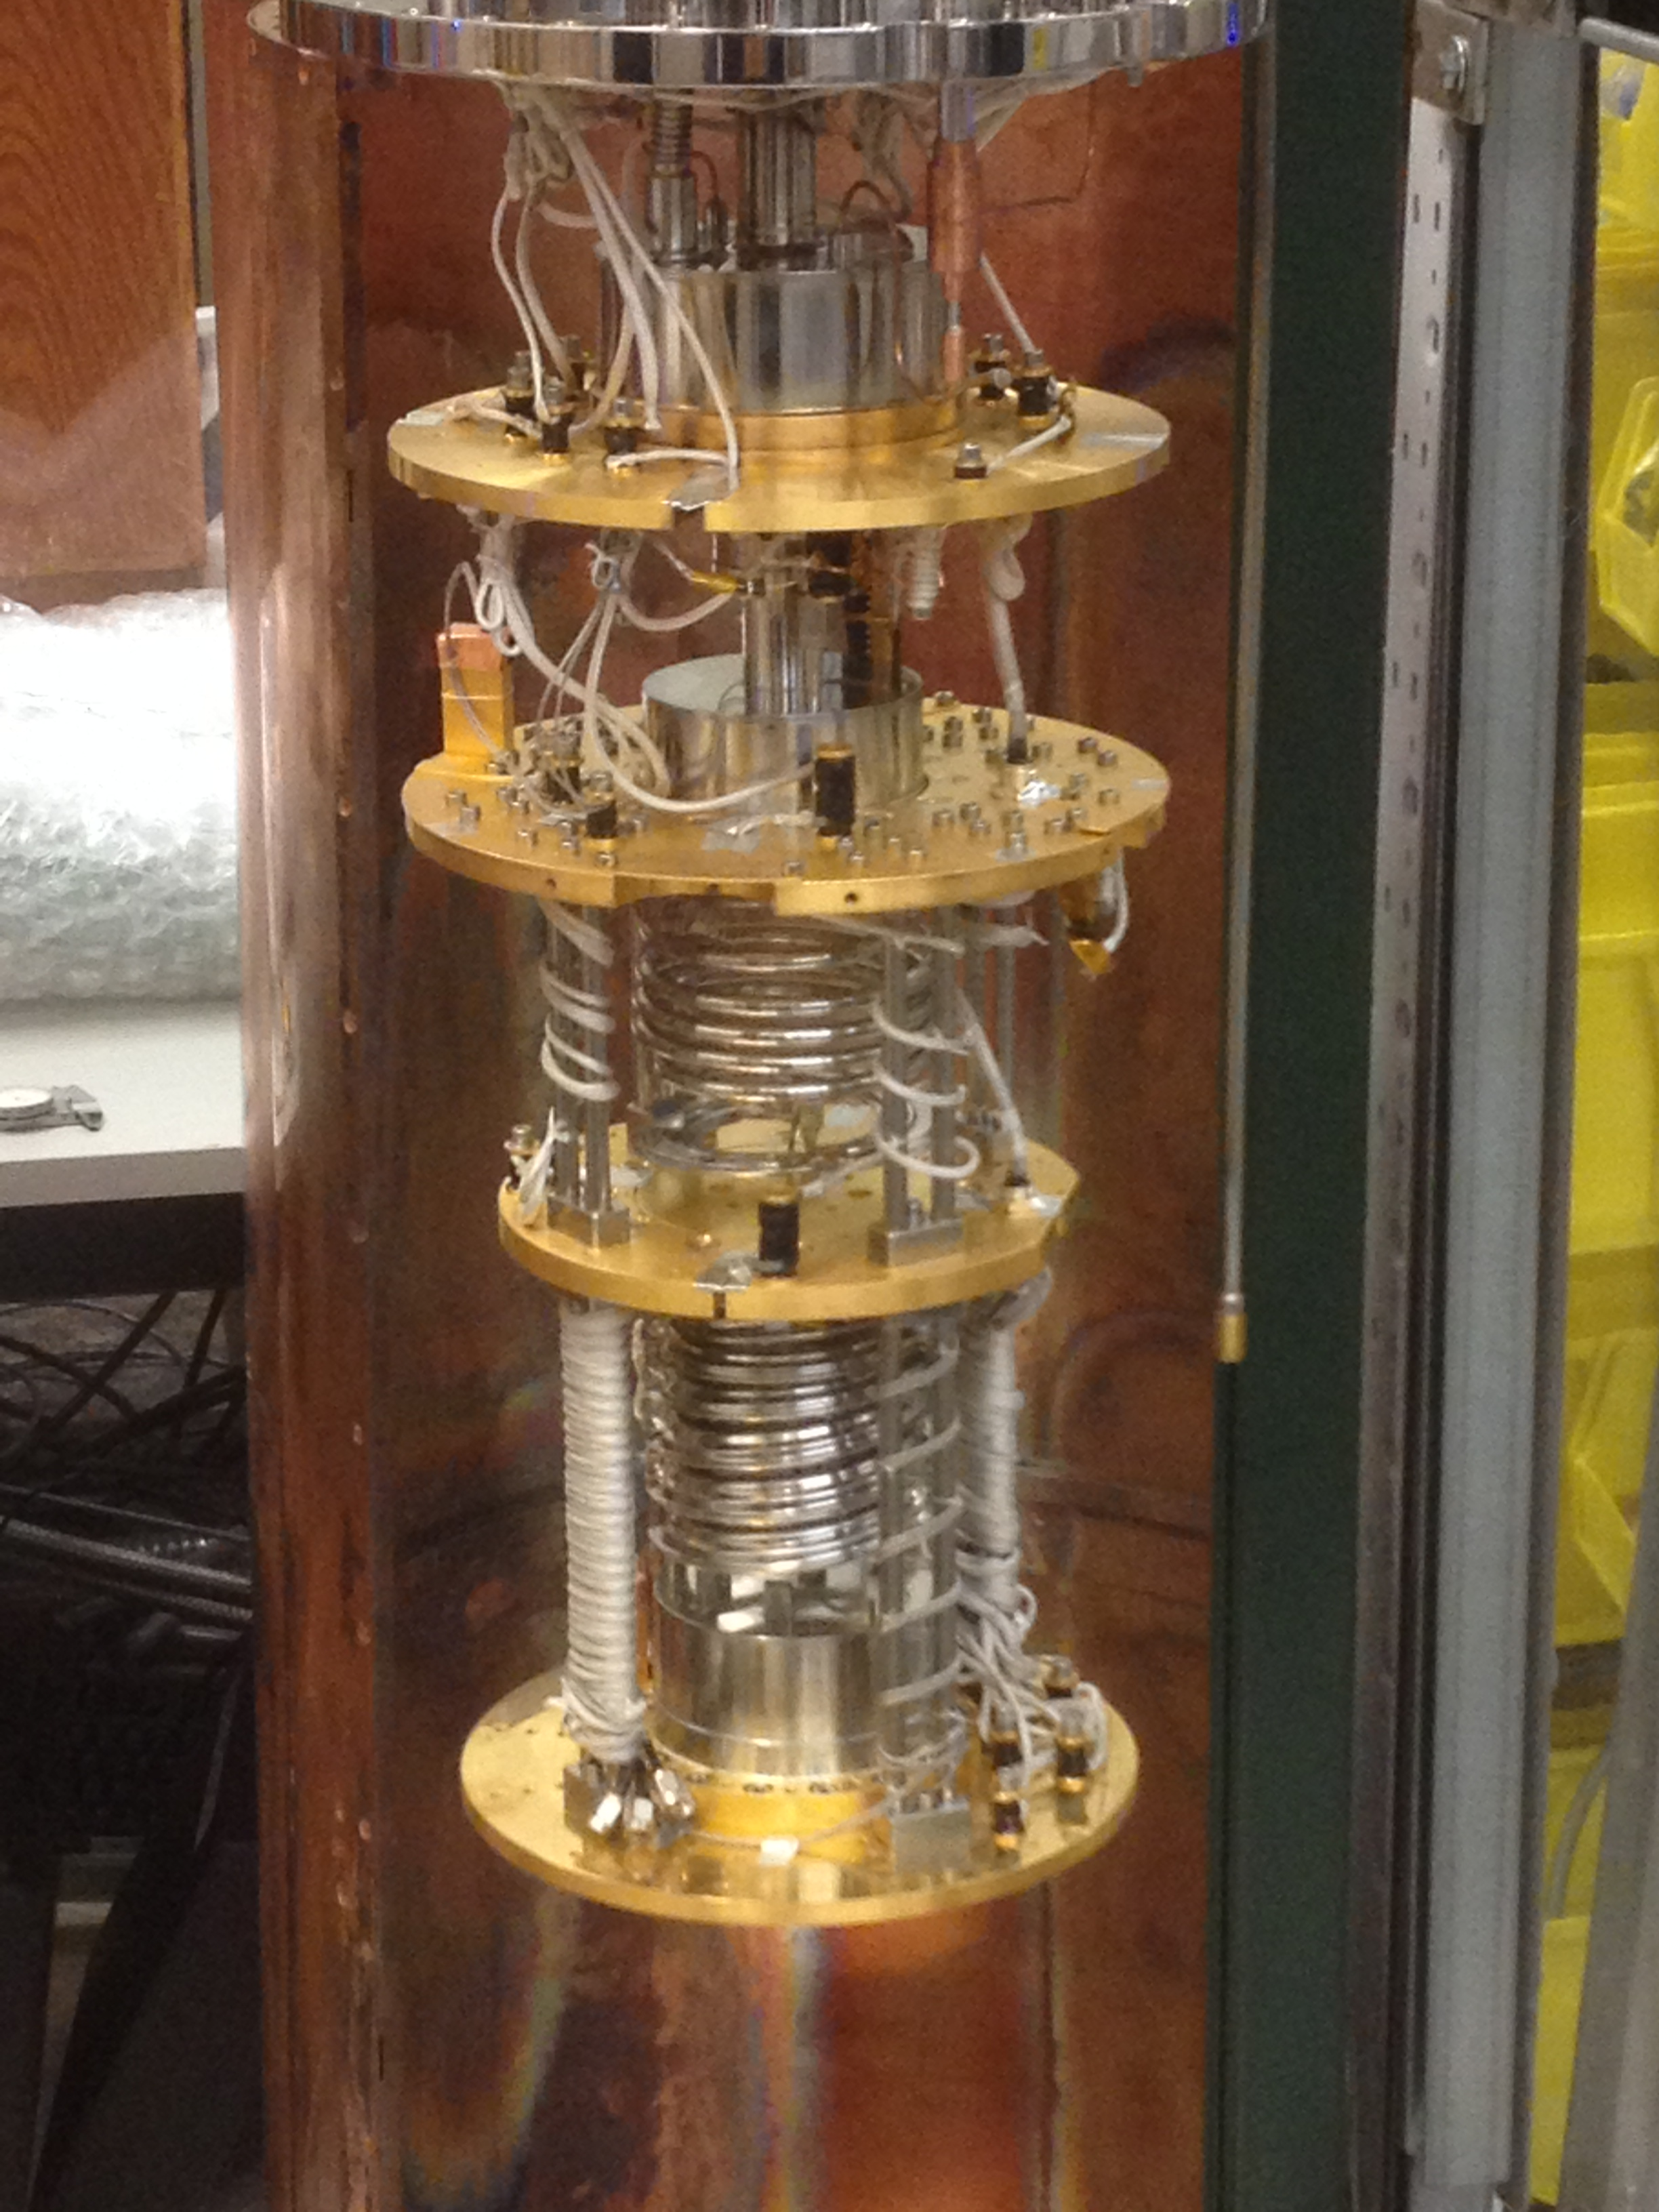
\includegraphics[width=0.5\textwidth]{dil_fridge_glamour_shot}
%
%\end{frame}


%\begin{frame}{Experimental Site Picture}
%\includegraphics[width=\textwidth]{boutan_photo13}
%\end{frame}

%\begin{frame}{Insert}
%houses quantum-limited amplifiers and cavity. goes in magnet.
%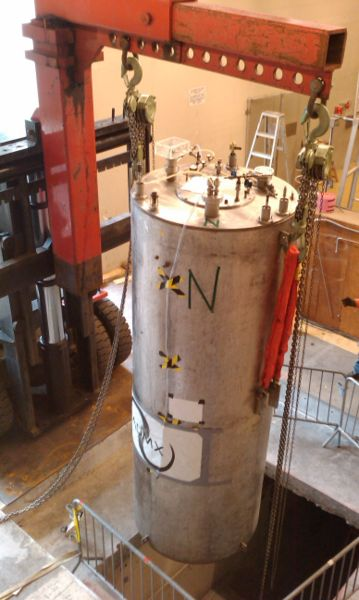
\includegraphics[width=0.5\textwidth]{magnet_lowered}
%\end{frame}

%\begin{frame}{Insert}
%houses quantum-limited amplifiers and cavity. goes in magnet.
%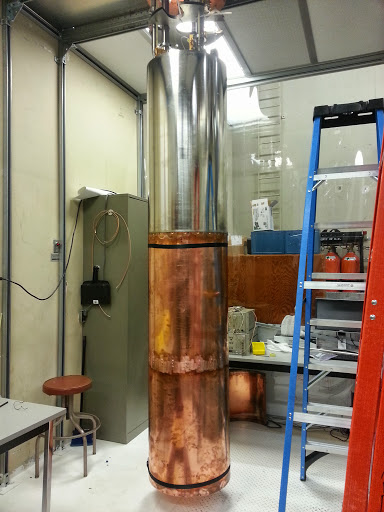
\includegraphics[width=0.5\textwidth]{cavity_buttoned_up}
%%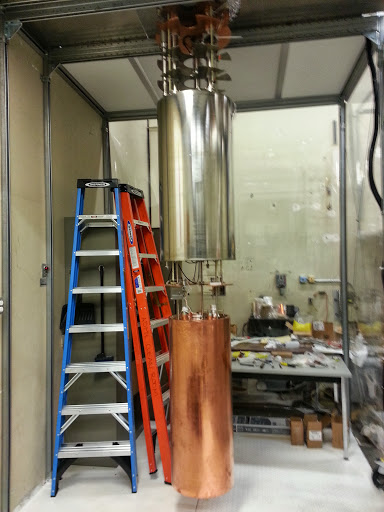
\includegraphics[width=0.5\textwidth]{cavity_hanging}
%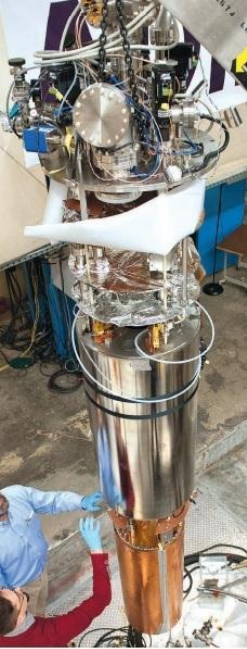
\includegraphics[width=0.3\textwidth]{insert_going_in}
%
%\end{frame}

%\begin{frame}
%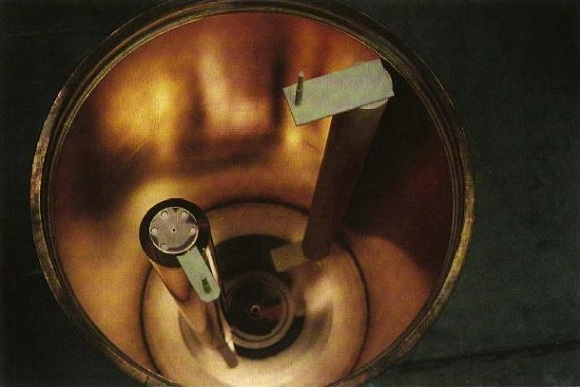
\includegraphics[width=0.5\textwidth]{cavity_open}
%\end{frame}


%\begin{frame}
%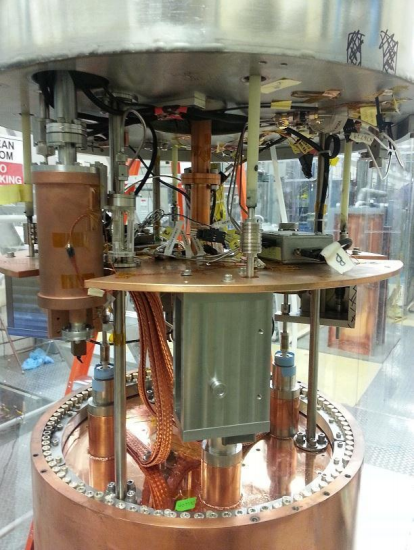
\includegraphics[width=0.4\textwidth]{another_1k_plate_pic}
%%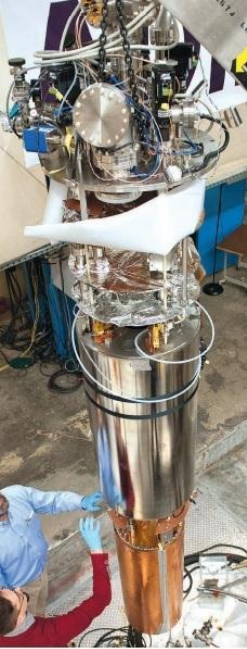
\includegraphics[width=0.3\textwidth]{insert_going_in}
%\end{frame}



%\begin{frame}
%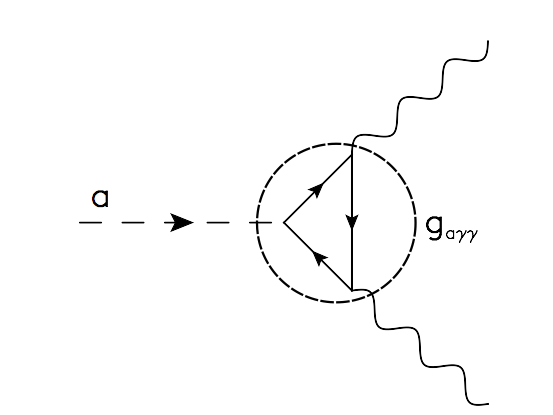
\includegraphics[width=0.5\textwidth]{axion_photon_feynman_diagram}
%\end{frame}

%\begin{frame}
%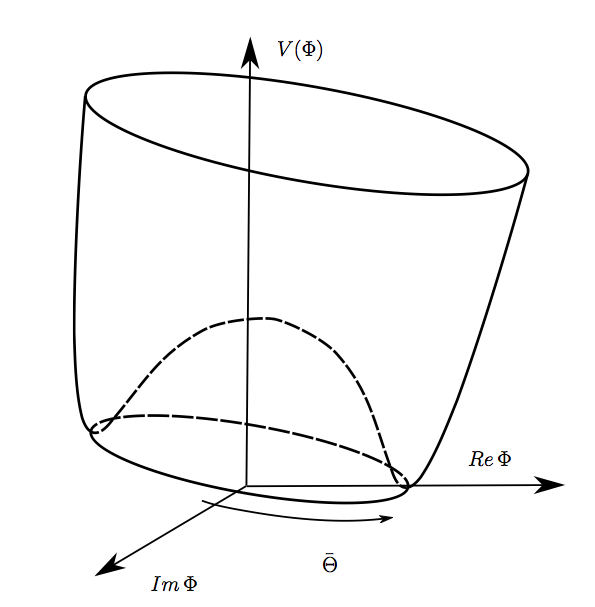
\includegraphics[width=0.5\textwidth]{wine_bottle}
%\end{frame}

%\begin{frame}
%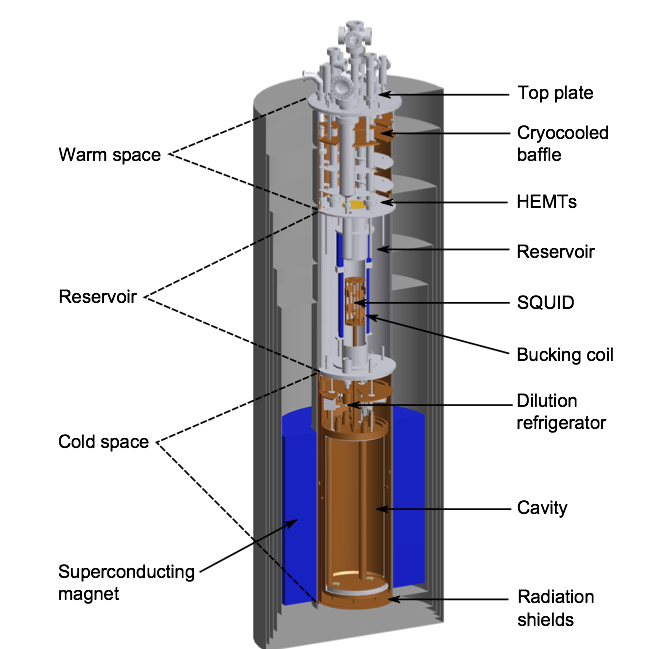
\includegraphics[width=0.5\textwidth]{schematic_with_labels}
%\end{frame}

%\begin{frame}
%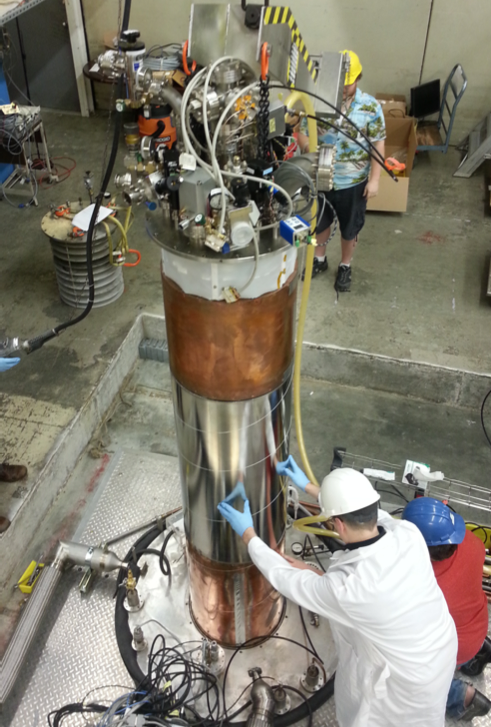
\includegraphics[width=0.5\textwidth]{lowering_insert}
%\end{frame}

%\begin{frame}
%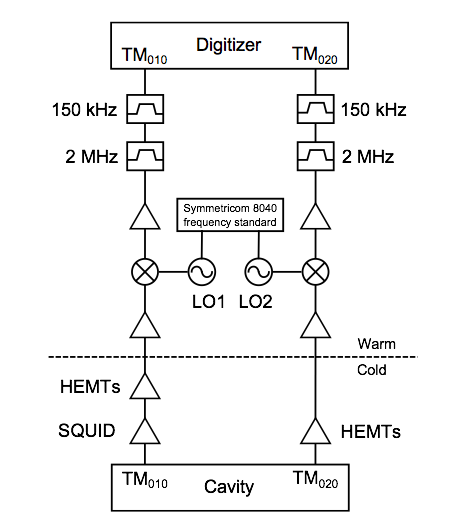
\includegraphics[width=0.5\textwidth]{two_channel_diagram}
%\end{frame}

%\begin{frame}
%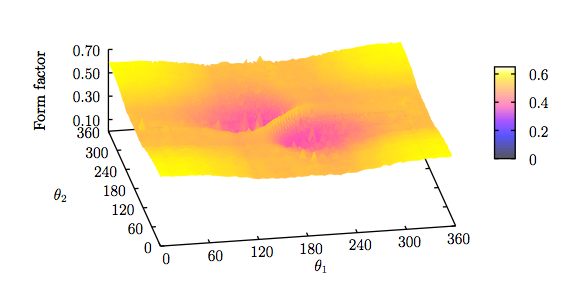
\includegraphics[width=0.5\textwidth]{2d_ff}
%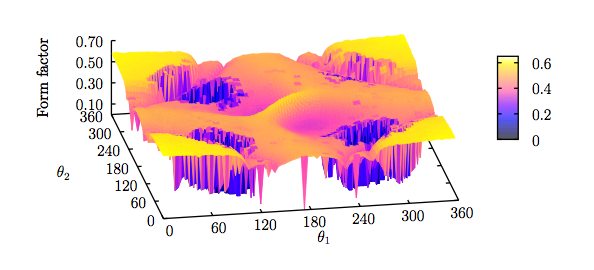
\includegraphics[width=0.5\textwidth]{3d_ff}
%\end{frame}

%\begin{frame}
%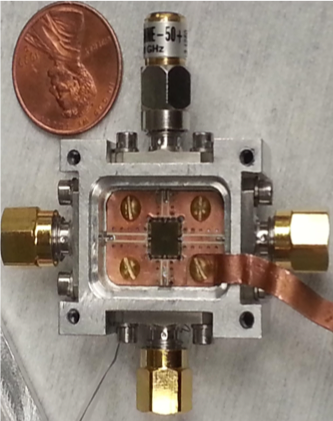
\includegraphics[width=0.5\textwidth]{jpa_exposed}
%\end{frame}

%\begin{frame}
%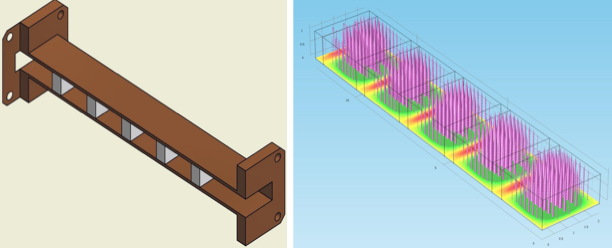
\includegraphics[width=0.5\textwidth]{dielectric_in_waveguide}
%\end{frame}


%\begin{frame}{Schedule}
%gloss over hard work - turn on dil fridge in two weeks. Start taking data end of summer.
%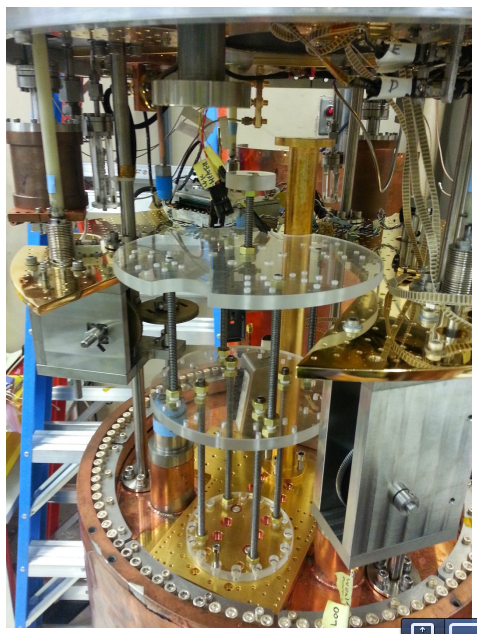
\includegraphics[width=0.5\textwidth]{dummy_dil_fridge}
%\end{frame}
%
%\begin{frame}{Most Recent Results - 2014 Data Run}
%Show Dima's plots. Tm020 and TM010 mode simultaneous running.
%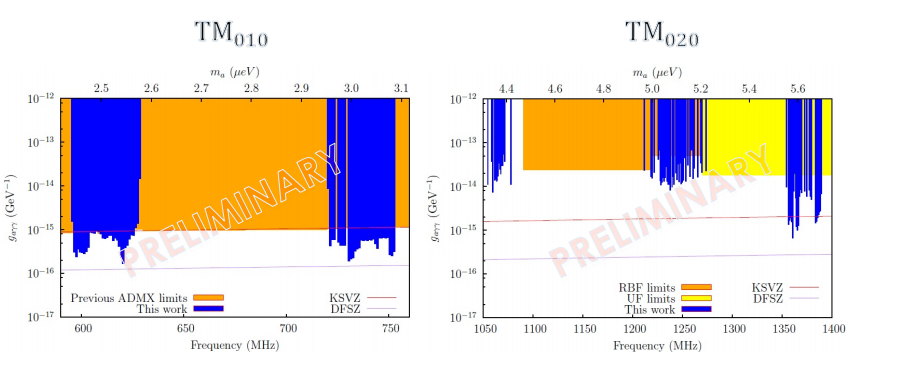
\includegraphics[width=\textwidth]{2014_results}
%
%\end{frame}

%\begin{frame}{New Things}
%operate JPA on second channel.
%sidecar. picture of sidecar. piezo motors.
%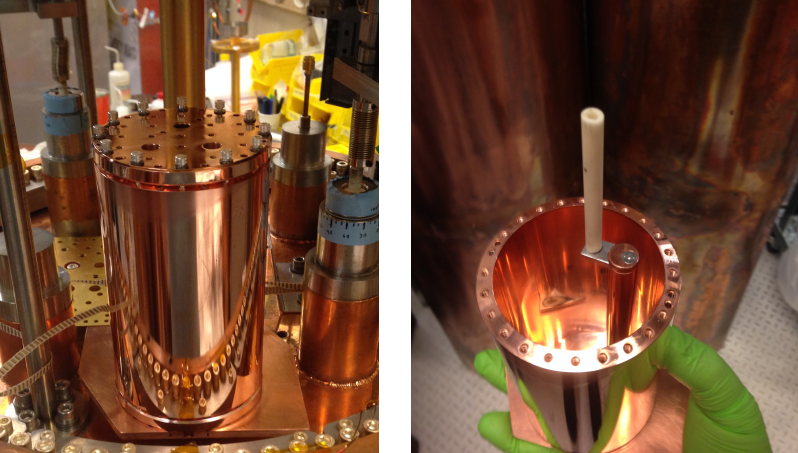
\includegraphics[width=\textwidth]{sidecar_duo}
%\end{frame}
%
%\begin{frame}{Technical Subtleties and what makes this a systematic free experiment}
%Subtleties:
%modeling gap in form factor.
%tuning and finding mode crossings.
%assumes dark matter density is some number.
%Why the Axion is Special:
%your signal is very hard to fake - it depends on B, Q, mode, cavity frequency. so although one sees
%statistical fluctuations, and there are environmental signals, one can always turn the magnetic field off and see if it
%persists.
%\end{frame}
%
%\begin{frame}
%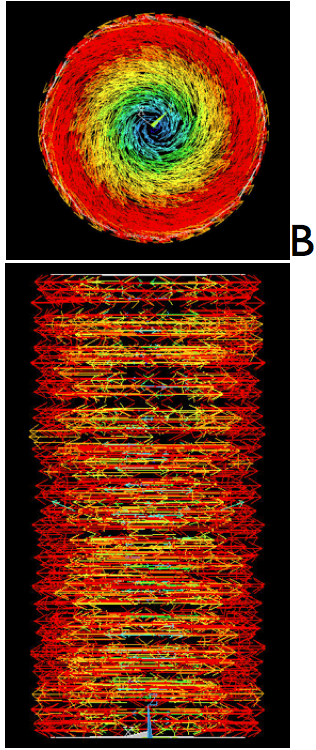
\includegraphics[width=0.5\textwidth]{empty_cavity_b}
%
%\end{frame}
%
%\begin{frame}
%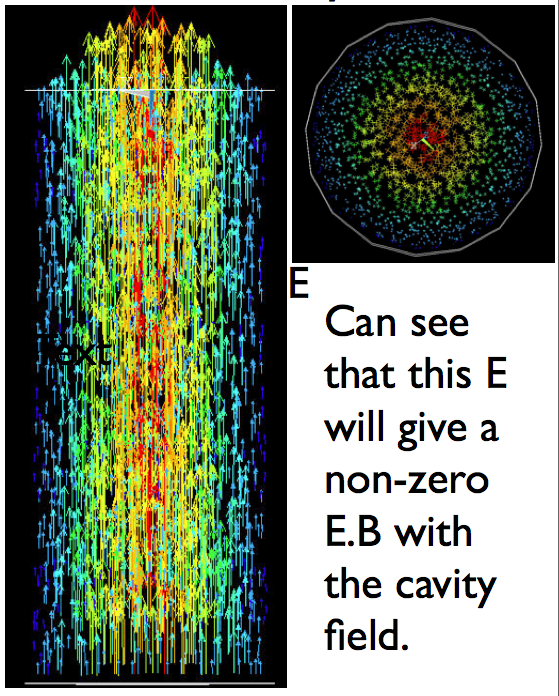
\includegraphics[width=0.5\textwidth]{empty_cavity_e}
%\end{frame}
%\begin{frame}
%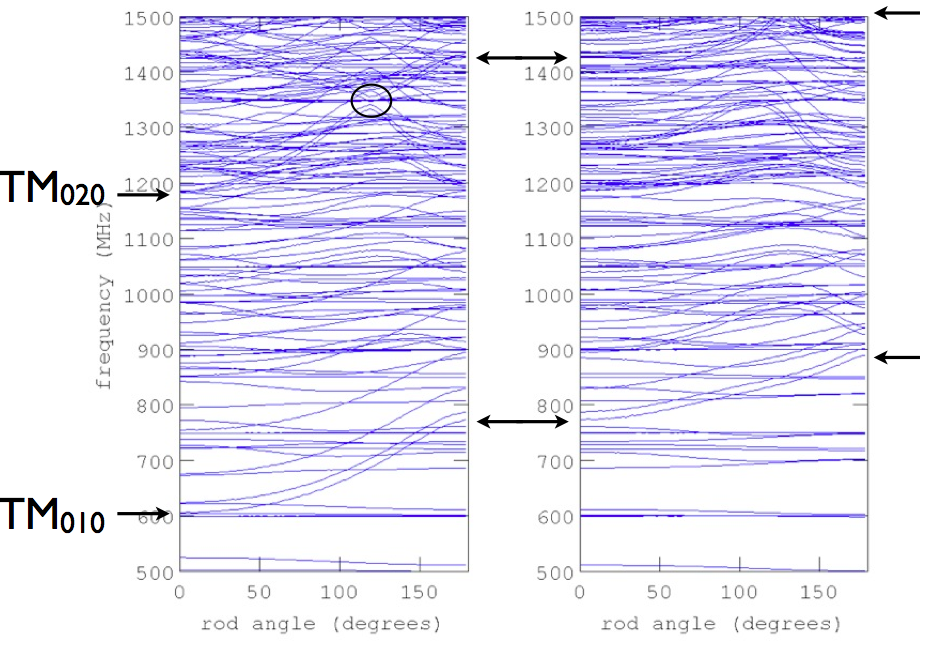
\includegraphics[width=0.5\textwidth]{daw_mode_map}
%
%\end{frame}

\begin{frame}{Research in Progress}
\begin{columns}
\column{0.5\textwidth}
{\tiny dielectric plates in waveguide}
\includegraphics[width=\textwidth]{dielectric_in_waveguide}
\vspace{10 mm}
{\tiny feedback}
\includegraphics[width=\textwidth]{delay}
\column{0.5\textwidth}
{\tiny sinusoidal magnetic field}
\includegraphics[width=\textwidth]{orpheus_duo}

{\tiny rectangular cavities}
\includegraphics[width=.8\textwidth]{rectangular_cavity}



\end{columns}
%why 3D cavities fail.
%how to fix it by allowing magnetic field to wiggle. Orpheus
%how to fix it by allowing electric field to not integrate to 0. (Electric Tiger, Aaaron's bendy thing)
%how to fix it by increasing Q. Ouroboros
%how to fix it by making rectangular cavities.
\end{frame}

%\begin{frame}{Idea}
%\begin{itemize}
%\item Axion haloscopes experiments use high-Q microwave cavities.
%
%\item Expected signal power is proportional to Q:
%\begin{align*}
%P_{sig} \propto \text{min}\big(Q_L, Q_a\big)
%\end{align*}
%axion quality factor: $Q_a \simeq 10^6$
%\item Theoretical Q goes as 
%\begin{align*}
%Q = \frac{L}{R+L}\frac{R}{\delta}
%\end{align*}
%
%\item anomalous skin depth (Cu): $\delta = 2.8\times10^{-5}\text{ cm}\bigg(\frac{\text{GHz}}{f}\bigg)^{1/3}$
%
%\item  $Q_L \approx 10^5$ for $f \approx 1$ GHz.
%
%
%\item Can we increase the loaded Q further? 
%\end{itemize}
%\end{frame}
%
%\begin{frame}{Introduce Feedback}
%\centering
%\includegraphics[width=\textwidth]{cavity_linear_to_nonlinear}
%
%\end{frame}

%\begin{frame}{Active Feedback}
%\centering
%\includegraphics[width=0.6\textwidth]{export_sparams_10}
%\end{frame}
%
%\begin{frame}{Active Feedback}
%\centering
%\includegraphics[width=0.65\textwidth]{export_sparams_4}
%\end{frame}

%\begin{frame}{Proposal}
%\centering
%\includegraphics[width=\textwidth]{arxiv_snapshot}
%
%\includegraphics[width=0.3\textwidth]{gray_headshot}
%\includegraphics[width=0.3\textwidth]{experiment_schematic-eps-converted-to}
%
%\footnotetext{arXiv:1403.6720}
%\end{frame}

%\begin{frame}{Active Feedback}
%{$V_{out} = V_{in}S_{21}(1 + x + x^2 + \ldots) = V_{in}S_{21}(1-x)^{-1}$}
%\begin{columns}
%\column{0.65\textwidth}
%\centering
%\includegraphics[width=\textwidth]{nonlinear_scaling}
%\column{0.35\textwidth}
%\begin{itemize}
%\item Signal builds up through feedback 
%\item Q increases by factor $(1-x)^{-1}$
%\item Oscillation begins when $x=1$
%\end{itemize}
%\end{columns}
%\end{frame}

%\begin{frame}{Active Feedback}
%\centering
%\includegraphics[width=0.65\textwidth]{export_sparams_7}
%\end{frame}
%
%\begin{frame}{Active Feedback}
%\centering
%\includegraphics[width=0.65\textwidth]{export_sparams_8}
%\end{frame}
%
%\begin{frame}{Active Feedback}
%\centering
%\includegraphics[width=0.65\textwidth]{export_sparams_9}
%\end{frame}
%
%
%\begin{frame}{Active Feedback}
%\centering
%\includegraphics[width=0.65\textwidth]{export_sparams_13}
%\end{frame}
%
%\begin{frame}{Active Feedback}
%\centering
%\includegraphics[width=0.65\textwidth]{export_sparams_14}
%\end{frame}

%\begin{frame}
%\begin{itemize}
%\item This idea is old; patented in 1914 and used for making higher gain amplifiers and more selective radio circuits.\footnote{Joe A. Rolf, "Q Multiplier Boosts Selectivity $\&$ Gain," Popular Electronics, April 1974} 
%
%\item However, this amplifies noise and signal equally, so SNR should remain the same for constant amplitude signal:
%\begin{align*}
%\text{SNR}_{\text{cw}} \propto \text{const.}
%\end{align*}
%\item Since axion signal is proportional to $Q$, SNR increases
%\begin{align*}
%\text{SNR}_{\text{axion}} \propto (1-x)^{-1}
%\end{align*}
%\item We can utilize the different coherence times of signal and noise to get more improvement.
%\end{itemize}
%\end{frame}

%\begin{frame}{Time Delay}
%{\tiny Introduce a time delay so $t_0$ greater than cavity coherence time}
%\begin{columns}
%\column{0.6\textwidth}
%\centering
%\includegraphics[width=\textwidth]{delay}
%\column{0.4\textwidth}
%\begin{itemize}
%\item Noise is only correlated over time $t_{cav}$
%\item Signal is coherent over longer time $t_{a}$
%\item If roundtrip time $t_0$ is greater than $t_{cav}$:
%\begin{align*}
%t_{cav} < t_0 < t_a
%\end{align*}
%we expect noise to add incoherently and signal
%to add coherently
%
%\end{itemize}
%\end{columns}
%\end{frame}

%\begin{frame}{Expected Improvement in Axion SNR}
%{\tiny axion snr improvement, $\text{SNR}(x)/\text{SNR}(x=0)$, with and without delay line}
%\includegraphics[width=\textwidth]{delay_no_delay}
%\end{frame}

%\begin{frame}{Expected Improvement in Constant Signal}
%{\tiny cw snr improvement, $\text{SNR}(x)/\text{SNR}(x=0)$,  with and without delay line}
%\includegraphics[width=\textwidth]{looking_at_coth}
%\end{frame}

\begin{frame}{Initial Setup}
{\tiny feedback using amplifiers, variable attenuator, and phase shifter}
\includegraphics[width=\textwidth]{first_circuit_no_delay}
\end{frame}

\begin{frame}{Q Enhancement}
{\tiny adjusting variable attenuator allows $Q$ to range from 1000 to 9000 before oscillations begin}
\includegraphics[width=0.5\textwidth]{low_q}
\includegraphics[width=0.5\textwidth]{high_q}
\end{frame}

%\begin{frame}{Setup}
%\includegraphics[width=\textwidth]{first_circuit_version}
%\end{frame}

%\begin{frame}{Active Feedback Resonator}
%{\tiny Ouroboros}
%%\begin{columns}
%%\column{0.5\textwidth}
%\includegraphics[width=\textwidth]{export_ouroboros}
%%\column{0.5\textwidth}
%%\begin{itemize}
%%\item $t$: time around loop
%%\item $\tau$: coherence time of cavity
%%\item Intuition: signal feeds back coherently; when $t > \tau$, noise adds incoherently
%%\end{itemize}
%%\end{columns}
%\end{frame}

\begin{frame}{Schematic}
\includegraphics[width=\textwidth]{no_isolator}
\end{frame}


%\begin{frame}{Parameters}
%\begin{columns}
%\column{0.5\textwidth}
%\begin{tabular}{| l l |}
%\hline
%Parameter & Values \\
%\hline
%\hline
%$f_{\text{cav}}$ & 2.256 GHz \\ 
%$t_{\text{delay}}$ & 2.4 $\mu$s \\
%$t_{\text{cav}}$ & 170 ns \\ 
%$t_{\text{axion}}$ & 141 $\mu$s \\
%\hline
%\end{tabular}
%\column{0.5\textwidth}
%Experiment
%\begin{itemize}
%\item Set attenuation of variable attenuator
%\item Adjust phase so Q is maximal
%\item Measure Q, $f_{cav}$
%\item Inject constant amplitude signal at $f_{cav}$
%\item Measure height of signal relative to noise floor in detected spectrum
%\end{itemize}
%\end{columns}
%\end{frame}

%\begin{frame}{Axion and CW Signal}
%{\tiny Scenario 1}
%\includegraphics[width=\textwidth]{first_limit}
%
%\end{frame}
%
%\begin{frame}{Axion and CW Signal}
%{\tiny Scenario 2}
%\includegraphics[width=\textwidth]{second_limit}
%\end{frame}
%
%\begin{frame}{Axion and CW Signal}
%{\tiny Scenario 3}
%\includegraphics[width=\textwidth]{third_limit}
%\end{frame}


%\begin{frame}{Exploring Second Limit}
%{\tiny$t_1 \ll t_{cav}$}
%\includegraphics[width=\textwidth]{exploring_second_limit_low}
%\end{frame}
%
%\begin{frame}{Exploring Second Limit}
%{\tiny $t_1 > t_{cav}$}
%\includegraphics[width=\textwidth]{exploring_second_limit_high}
%\end{frame}

%\begin{frame}{Theory and Experiment}
%{Comparison}
%\includegraphics[width=\textwidth]{comparison_xaxis_gain}
%\end{frame}


%\begin{frame}{Active Feedback Resonator}
%{\tiny Ouroboros}
%\begin{columns}
%\column{0.5\textwidth}
%\includegraphics[width=\textwidth]{experiment_schematic-eps-converted-to}
%\column{0.5\textwidth}
%\begin{itemize}
%\item $t$: time around loop
%\item $\tau$: coherence time of cavity
%\item Intuition: signal feeds back coherently; when $t > \tau$, noise adds incoherently
%\end{itemize}
%\end{columns}
%\end{frame}

%\begin{frame}{Equivalent Circuit}
%\centering
%\includegraphics[width=.5\textwidth]{qmultiplier}
%
%$G_l$ the loop gain\\
%$Q_0$ the active quality factor\\
%$T_a$ the amplifier noise temperature\\
%%$T_{cav}$ the cavity noise temperature\\
%\begin{columns}
%\column{0.5\textwidth}
%\centering
%\begin{align*}
%Q_0 = Q_L(1-\sqrt{G_l})^{-1} \\
%|\hat{S}_{21}|^2 \propto (1- \sqrt{G_l})^{-2}
%\end{align*}
%\column{0.5\textwidth}
%\centering
%\begin{align*}
%T_{noise} = \frac{T_{cav} + G_l T_a}{1 + G_l - 2\sqrt{G_l}e^{-t/\tau - i\theta}}
%\end{align*}
%\end{columns}
%\end{frame}

%\begin{frame}{Prototype}
%\begin{columns}
%\column{0.5\textwidth}
%\includegraphics[width=\textwidth]{active_resonator_setup_photo}
%\column{0.5\textwidth}
%\includegraphics[width=\textwidth]{s21_no_delay}
%
%\includegraphics[width=\textwidth]{s21_delay}
%\end{columns}
%
%\end{frame}

\begin{frame}{Results}
\includegraphics[width=\textwidth]{experiment}

{\tiny need to understand thermal noise in circuit and effect of coherence times, phase.}
\end{frame}

%\begin{frame}{Considerations}
%\begin{itemize}
%\item analog delay lines are narrowband frequency devices - move to digital delay lines.
%\item major design considerations would center around gain instability; to get $10$x increase in Q, need $x \simeq 0.9$.
%\item amplifier saturation - our low noise SQUID saturates at 8K. If we have 100 mK system noise temperatures, but increase the Q by a factor of 10x, the noise power will increase by a factor of 100x.
%\end{itemize}
%\end{frame}
%
%\begin{frame}{Conclusions}
%\begin{itemize}
%\item active feedback is a simple technique to increase Q
%\item delay line provides additional increase in SNR
%\item independent of other parts of the experiment
%\item does not need to be operated cryogenically
%%\item phase shifter allows for fine tuning of resonance
%\end{itemize}
%\end{frame}
%
%
%\begin{frame}{People}
%{Lisa McBride, Kunal Patel, Gray Rybka}
%{\tiny This work was supported by the Dept. of Energy, Division of High Energy Physics.}
%
%\begin{columns}
%\column{0.5\textwidth}
%\includegraphics[width=0.8\textwidth]{lisa_pic}
%\includegraphics[width=\textwidth]{kunal_pic}
%
%\column{0.5\textwidth}
%\includegraphics[width=\textwidth]{gray_pic}
%
%\end{columns}
%
%\end{frame}

%\begin{frame}{Acknowledgments}
%DOE HEP
%\end{frame}


\begin{frame}{People}

{\tiny \textbf{Fermilab}
Aaron Chou

\textbf{LBNL}
Gianpaolo Carosi

\textbf{University of Washington}
Leslie Rosenberg
Gray Rybka
Christian Boutan
James Sloan
Cliff Plesha
Hannah LeTourneau
Rich Ottens
Kunal Patel
Kiva Ramundo
Jacob Herr
Xavier Frost
Ana Malagon

\textbf{University of Florida}
David Tanner
Neal Sullivan
Ian Stern
Nicole Crisosto
Joe Gleason

\textbf{Berkeley}
Irfan Siddiqi
Karl van Bibber
John Clarke
Sean O'Kelley

\textbf{Sheffield U}
Edward Daw

\textbf{NRAO}
Richard Bradley

\textbf{Previous Members}
Michael Hotz
Andrew Wagner
Dmitry Lyapustin
Jeffrey Hoskins
Leanne Duffy
Steve Asztalos
Darin Kinion
Danny Yu
Edward Daw
Christian Hagmann}
\end{frame}

\begin{frame}
\includegraphics[width=\textwidth]{dark_admx}
\end{frame}

%\begin{frame}{Backup}
%\centering
%Backup Slides
%\end{frame}
%
%\begin{frame}{If $Q_L > Q_a$}
%\includegraphics[width=0.5\textwidth]{axion_bw}
%
%If cavity Q is larger than axion Q (or $t_{cav} > t_a$), we no longer detect the full axion power within the cavity bandwidth.
%\end{frame}

%\begin{frame}{Delay Lines}
%{\tiny Surface Acoustic Wave (SAW) Resonator}
%\includegraphics[width=\textwidth]{saw}
%\end{frame}
%
%\begin{frame}{Expected SNR Improvement}
%{\tiny analysis of signal correlation}
%Scenario 1: $t_0 \ll t_{cav}$: .
%\begin{align*}
%\langle V_{in}(t)V_{in}(t-t_0)\rangle &= \bar{V}_{in}^2\\
%\langle|V_{out}|^2\rangle = |\bar{V}_{in}S_{21}|^2(1 + x + x^2 + \ldots)^2 &= \bar{V}_{in}^2|S_{21}|^2(1-x)^{-2}
%\end{align*}
%Scenario 2: $t_0 \sim \mathcal{O}(t_{cav})$:  
%\begin{align*}
%\langle V_{in}(t)V_{in}(t-t_0)\rangle &= \bar{V}_{in}^2e^{-t_0/t_{cav}}\\
%\langle|V_{out}|^2\rangle &=  |\bar{V}_{in}S_{21}|^2(1 + xe^{-t_0/t_{cav}} + x^2e^{-2t_0/t_{cav}} + \ldots)^2 \\
%&= \bar{V}_{in}^2|S_{21}|^2(1-xe^{-t_0/t_{cav}})^{-2}
%\end{align*}
%this analysis is not completely correct - it predicts a turnover at x=0.5. One needs to treat the nonlinearity properly to get the correct result:
%\begin{align*}
%\langle|V_{out}|^2\rangle = \frac{\bar{V}_{in}^2|S_{21}|^2}{(1-x)^{2}}\frac{1 + xe^{-t_0/t_{cav}}}{1 - xe^{-t_0/t_{cav}}}
%\end{align*}
%\end{frame}

%\begin{frame}{Comparison (preliminary)}
%\includegraphics[width=\textwidth]{comparison_xaxis_gain}
%\end{frame}

%\begin{frame}{Interference Fringes}
%When $\Delta f t_0 > \pi$, one sees interference fringes, due to off resonant signals acquiring an extra phase shift of $\pi/2$ relative to the phase acquired by the resonant frequency.
%\includegraphics[width=\textwidth]{s21_delay}
%\end{frame}

\end{document}